\documentclass[10pt]{article}
\usepackage[margin=15mm]{geometry}
\usepackage{amsmath,amssymb,tikz,pgfplots}
\pgfplotsset{compat=1.18}
\definecolor{digitZero}{HTML}{246C91}
\definecolor{digitOne}{HTML}{BC632E}
\pagestyle{empty}
\begin{document}
\begin{center}
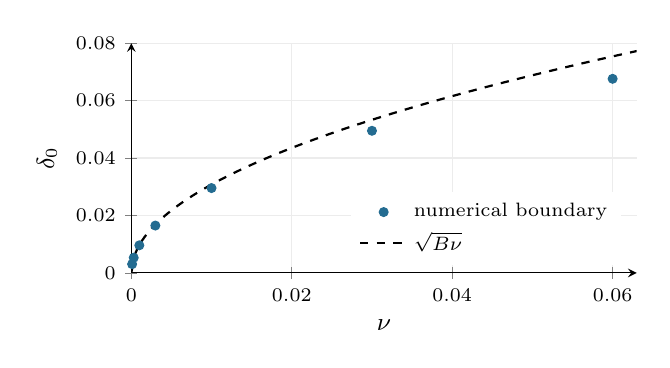
\begin{tikzpicture}
\begin{axis}[height=4.5cm,scale only axis=false,
 axis lines=left,tick label style={font=\scriptsize},label style={font=\small},
 title style={font=\small},legend style={font=\scriptsize,draw=none,fill=white},
 legend cell align=left,scaled ticks=false,grid=major,grid style={gray!15},
 tick label style={/pgf/number format/use period,/pgf/number format/fixed,/pgf/number format/precision=3,font=\scriptsize},width=8cm,xmin=0,xmax=.063,ymin=0,ymax=.08,
 xlabel={$\nu$},ylabel={$\delta_0$},
 xtick={0,.02,.04,.06},ytick={0,.02,.04,.06,.08},legend pos=south east]
\addplot[only marks,mark=*,mark size=1.6pt,digitZero] coordinates {(0.0001,0.00306548319808) (0.0003,0.00529467035476) (0.001,0.00961225037959) (0.003,0.016494421264) (0.01,0.0295381889851) (0.03,0.0494825785851) (0.06,0.0675831803396)};
\addlegendentry{numerical boundary}
\addplot[black,dashed,thick,domain=0:.063,samples=151] {sqrt((.5-4/pi^2)*x)};
\addlegendentry{$\sqrt{B\nu}$}
\end{axis}
\end{tikzpicture}
\end{center}\end{document}
